\subsubsection{Registrazione e Login}

\begin{scenario}{Scenario: Registrazione e Login}
  Ho deciso di iscrivermi a BrainBox per gestire meglio il mio studio.
  Una volta aperta la pagina di registrazione, noto subito che \textbf{non avendo un indicatore di avanzamento, non so quanti
  passaggi manchino} per completare il profilo.

  Inizio inserendo i dati personali e scelgo una password. In questa fase, mi
  accorgo che \textbf{non posso visualizzare i caratteri digitati} e quindi non posso verificare se ho scritto correttamente la password. Infatti, dopo aver confermato, compare un \textbf{messaggio d'errore in lingua inglese}, che mi risulta fuori luogo
  rispetto al resto dell'interfaccia in italiano.

  Superata questa fase, passo ai dettagli accademici. Aprendo il menu a tendina
  per l'ateneo, noto che \textbf{la voce} \textit{«Seleziona la tua università»} \textbf{è
  elencata come se fosse un'opzione selezionabile}, e lo stesso accade per i
  campi \textit{«Dipartimento»} e \textit{«Ciclo di studi»}.

  Qualche giorno dopo, provo a effettuare il Login. Anche in questo caso, digito con cautela la password dato che \textbf{non ho la possibilità di visualizzarla}. Sbaglio un carattere e appare nuovamente un \textbf{avviso in inglese}.

  Scopro inoltre che, sia nella fase di Registrazione sia nella fase di Login, \textbf{se volessi tornare alla Homepage o al passaggio precedente, per correggere un dato o annullare l'operazione, non c'è alcuna possibilità} se non cliccando dal tasto \textit{«Torna indietro»} del browser.
\end{scenario}

\paragraph{Design pattern applicati}
\begin{itemize}
  \item \textbf{Wizard + Modal Panel + Progress Indicator} (Tidwell): Il flusso di registrazione era già strutturato parzialmente come un wizard, un componente che guida l'utente passo dopo passo in un ordine prestabilito, indicato per task lunghi o complessi che l'utente affronta raramente, come la creazione di un profilo. L'intero wizard è presentato come un pannello sovrapposto all'interfaccia, concentrando l'attenzione dell'utente esclusivamente sul processo di registrazione senza distrazioni. Tramite questo pattern è stata aggiunta la possibilità di navigare liberamente tra gli step con un pulsante \textit{Indietro}, senza perdere i dati già inseriti. È inoltre possibile abbandonare l'operazione in qualsiasi momento tramite \textit{due link} (uno che porta alla pagina di Login/Registrazione e un altro che porta alla Homepage). Per quanto riguarda gli step, è stato seguito il pattern Progress Indicator, che prevede di mostrare su ogni pagina del wizard una mappa degli step con un indicatore, così l'utente sa esattamente dove si trova e quanto manca alla fine.

    Problemi di usabilità risolti:
    \begin{itemize}
      \item P10 (Non è possibile tornare alla homepage): è stato aggiunto un link, nella parte inferiore dei form di Registrazione e Login, che porta direttamente alla homepage.
      \item P54 (Nessun indicatore di progresso nel form di Registrazione): sono stati inseriti degli step per indicare all'utente a che punto si trova durante il processo di Registrazione.
    \end{itemize}

  \item \textbf{Password Strength Meter} (Tidwell): E' stato applicato questo pattern per permettere all'utente di avere un'idea chiara della robustezza della password che sta inserendo ed evitare di fargli fare molti tentativi prima di inserirla nel formato consentito. Inoltre, per supportare l'utente nella scelta e nell'inserimento della password, è stata adottata la soluzione indicata all'interno di questo pattern: rendere visibile un \textit{toggle} che consente di visualizzare i caratteri digitati. Come indicato dal pattern, il campo password non dovrebbe mostrare i caratteri di default, ma offrire all'utente la possibilità di farlo tramite un'apposita opzione. (Figura \ref{fig:registrazione_2})

    Problemi di usabilità risolti:
    \begin{itemize}
      \item P18 (Non è possibile visualizzare la password inserita): è stato aggiunto un toggle (occhiolino) per mostrare/nascondere la password inserita.
    \end{itemize}

  \item \textbf{Error Messages} (Tidwell): Il pattern prevede che i messaggi di errore siano posizionati direttamente nel form, vicino al campo che li ha generati, e scritti in linguaggio comprensibile per l'utente. Nel caso di BrainBox, i messaggi di errore apparivano in lingua inglese in un'interfaccia in italiano. La soluzione adottata è stata quella di tradurre i messaggi in italiano, rendendoli coerenti con il resto dell'interfaccia.

    Problemi di usabilità risolti:
    \begin{itemize}
      \item P9 (Il testo nei form di login e registrazione è in inglese): è stato tradotto il testo, compresi i messaggi di errore.
    \end{itemize}
\end{itemize}

\begin{figure}[H]
    \centering
    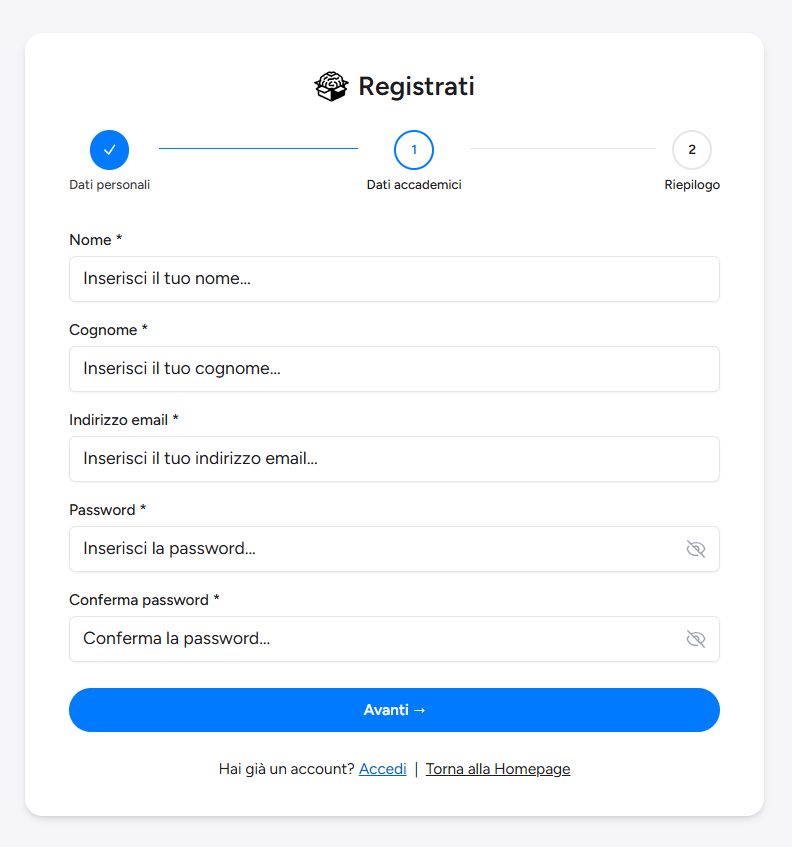
\includegraphics[width=0.6\textwidth]{figures/fig-riprogettazione-fisica/registrazione-login/registrazione_1.png}
    \caption{Step 1 Registrazione}
    \label{fig:registrazione_1}
\end{figure}

\begin{figure}[H]
    \centering
    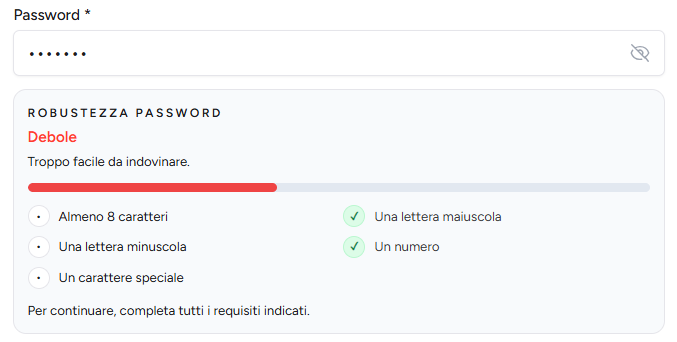
\includegraphics[width=0.6\textwidth]{figures/fig-riprogettazione-fisica/registrazione-login/registrazione_2.png}
    \caption{Controllo robustezza password}
    \label{fig:registrazione_2}
\end{figure}

\begin{figure}[H]
    \centering
    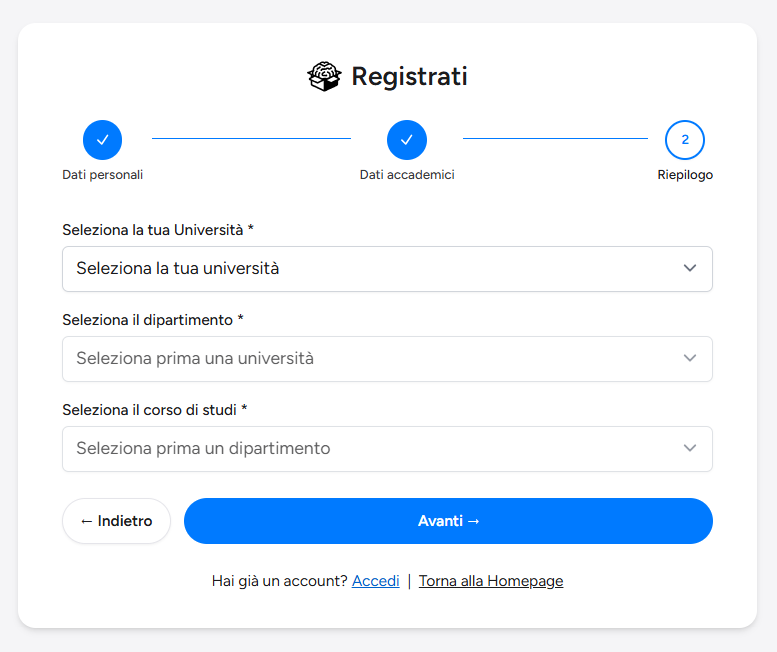
\includegraphics[width=0.6\textwidth]{figures/fig-riprogettazione-fisica/registrazione-login/registrazione_3.png}
    \caption{Step 2 Registrazione}
    \label{fig:registrazione_3}
\end{figure}

\begin{figure}[H]
    \centering
    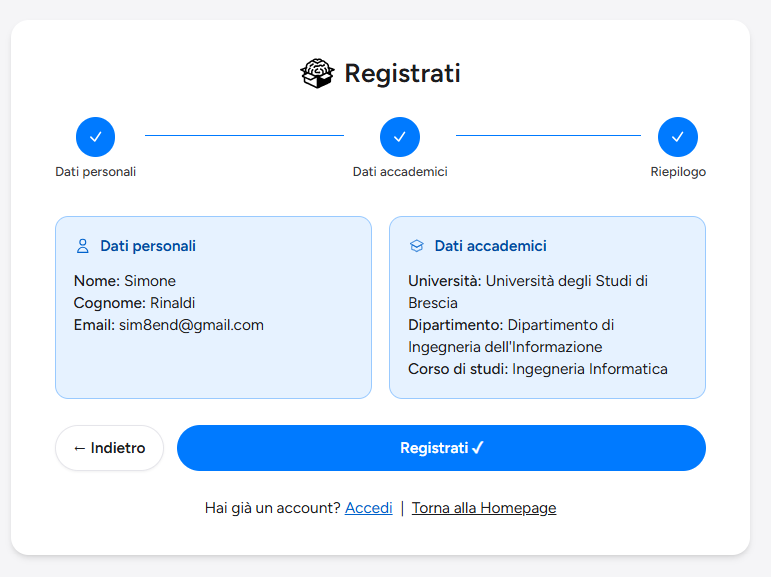
\includegraphics[width=0.6\textwidth]{figures/fig-riprogettazione-fisica/registrazione-login/registrazione_4.png}
    \caption{Step 3 Registrazione}
    \label{fig:registrazione_4}
\end{figure}

\begin{figure}[H]
    \centering
    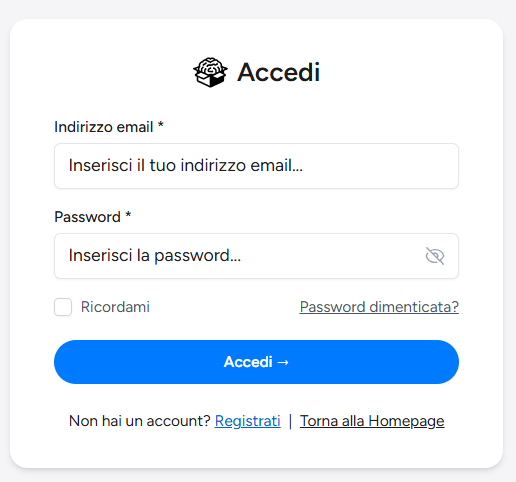
\includegraphics[width=0.6\textwidth]{figures/fig-riprogettazione-fisica/registrazione-login/accedi_1.png}
    \caption{Modale Accedi}
    \label{fig:accedi_1}
\end{figure}